%           - Header-           %
\documentclass[a4paper, 11pt, fleqn, notitlepage, egregdoesnotlikesansseriftitles]{scrartcl}
\usepackage[english, ngerman]{babel}                % Sprache: Deutsch
\usepackage[utf8]{inputenc}                         % Dateiformat
\usepackage[T1]{fontenc}                            % Schriftsatz

%       - wichtige Pakete -     %
\usepackage{kpfonts}                                % Schrift
\usepackage{geometry}                               % Struktur
\usepackage{hyperref}                               % klickbare links
\usepackage{amsmath, amssymb, mathtools}            % mathematische Formeln
\usepackage[headsepline]{scrlayer-scrpage}          % Kopf- und Fußzeilen konfigurieren

%       - nuetzliche Pakete -   %
%\usepackage{tabularx}                              % schöne tabellen
%\usepackage{booktabs}                              % Trennlinien in Tabellen
%\setlength{\columnsep}{0.7cm}                      % Spaltenabstand
%\usepackage{multicol}                              % mehrspaltiger Text
\usepackage{graphicx}                               % Grafiken
\usepackage[section]{placeins}
%\usepackage{tikz}                                  % Grafiken und Graphen
%\usepackage{diagbox}                               % Tabellen unterteilen
%\usepackage{bussproofs}                            % Logik und Kalkuele
%\usepackage{nicefrac}                              % schraege Brüche

% BibLateX
%\usepackage[backend=biber, authordate, eprint=false, url=false, block=ragged, bibencoding=inputenc]{biblatex-chicago}
%\usepackage{csquotes}
%\bibliography{quellen}                             % Quellen

%       - Eigene Befehle -      %
\newcommand{\emptyline}{\vspace{\baselineskip}}     % erzeugt leerzeile

%\newcommand{\N}{\mathbb{N}}
%\newcommand{\Z}{\mathbb{Z}}
%\newcommand{\R}{\mathbb{R}}
%\newcommand{\C}{\mathbb{C}}
%\newcommand{\Pf}{\mathbb{P}}

\newcommand{\aufgabe}{Block 6}
\newcommand{\modul}{Rechnernetze und Verteilte Systeme}
\newcommand{\sem}{Wintersemester 19/20}
\newcommand{\autorA}{Chunyu Zhou 380873}
\newcommand{\autorB}{Junyi Chen 390368}
\newcommand{\autorC}{Hongzhe Wang 383127}
\newcommand{\autoren}{Zhou, Chen, Wang}
\newcommand{\uni}{Technische Universität Berlin}
\newcommand{\datum}{\today}

%       - Einstellungen -       %
\title{\aufgabe}
\subtitle{\modul}
\author{\name}
\date{\datum}

%\setlength{\parindent}{0pt}                                        % einruecken verhindern
\pagestyle{scrheadings}
%\setcounter{secnumdepth}{0}                                        % keine Nummerierung von Überschriften
\geometry{left=25mm,right=20mm, top=27mm, bottom=25mm}              % bestimmte Seitenraender

\ihead{\aufgabe}
\chead{}
\ohead{\autoren}

\begin{document}

%         - Ttielseite -        %
%\maketitle
\thispagestyle{scrplain}

\noindent\Large
\textbf{\aufgabe} \hfill \textbf{\modul} \\
\normalsize
\autorA \hfill \uni \\
\autorB \hfill \sem \\
\autorC \hfill \datum \\
\autorD \hfill T18 G01 \\
\rule{\textwidth}{0.1mm}

%     - Inhaltsverzeichnis -    %
%\tableofcontents
%\newpage

%            - Text -           %

\section*{Ausgewählte Zeitserver}

Genutzte Servers:
\begin{itemize}
    \item 0.de.pool.ntp.org
    \item 1.de.pool.ntp.org
    \item 2.de.pool.ntp.org
    \item 3.de.pool.ntp.org
\end{itemize}

\emptyline
Für jeden Server wurden 100 aufeinander folgende Messungen mit 8 Sekunden Abstand gemacht.
Bei jeder Messung wurde dabei als Client ein NTP-Paket der Version 4 verschickt und die Antwort vom Server empfangen. Die Messungen der verschiedenen Server wurden sequentiell ausgeführt, sind also voneinander zeitlich unabhängig. Die Daten wurden in einer .txt Datei gesammelt und dann mittels der \verb+python3+ Bibliothek \verb+matplotlib+ graphisch veranschaulicht. Die Abbildungen mit der meisten Aussagekraft haben wir ausgewählt und in diesem Dokument dargestellt.

\newpage
\section*{Plots nach Offset, Delay und Root Dispersion}
\vspace{-\baselineskip}

\begin{center}
    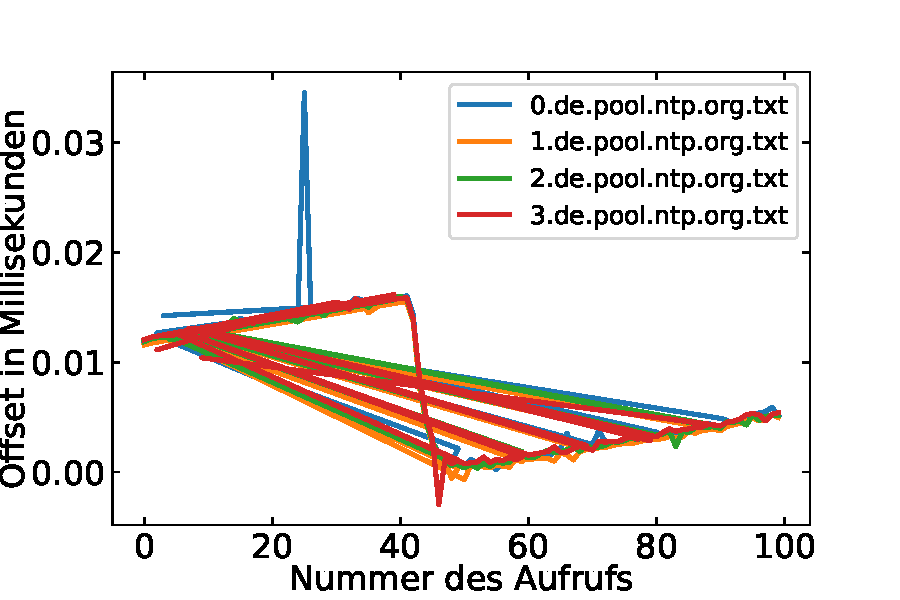
\includegraphics[width=\textwidth]{Offset_all.pdf}
    \captionof{figure}{Offset von allen Zeitservern}
    \label{fig:offset}
\end{center}

Aufgrund der großen Entfernung gibt es wesentlich mehr Knotenpunkte über die das Paket geleitet werden kann und somit viele verschiedene Routen mit unterschiedlichen Offsets.

\begin{center}
    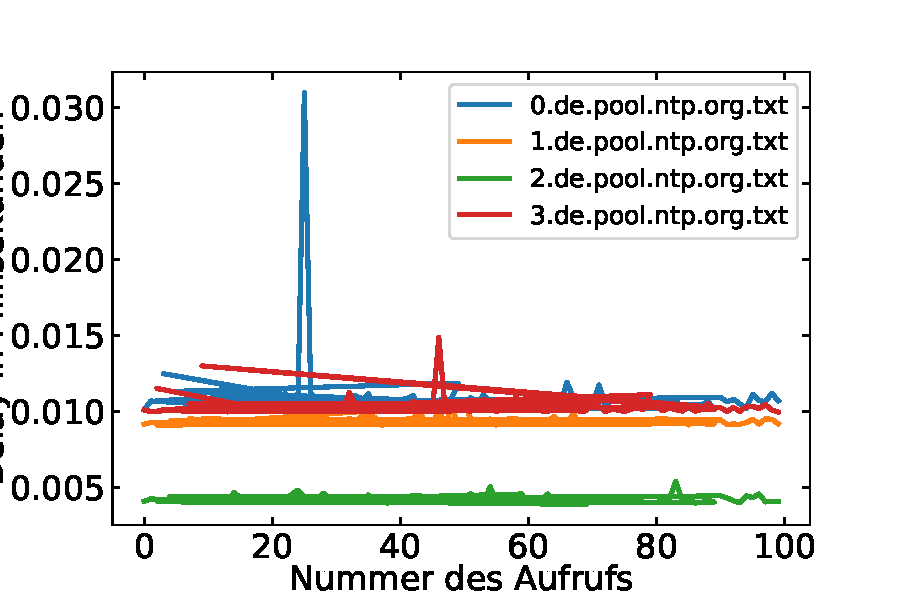
\includegraphics[width=\textwidth]{Delay_all.pdf}
    \captionof{figure}{Delay von allen Zeitservern}
    \label{fig:delay}
\end{center}

Das Delay ist dem Standort der Server entsprechend.

\begin{center}
    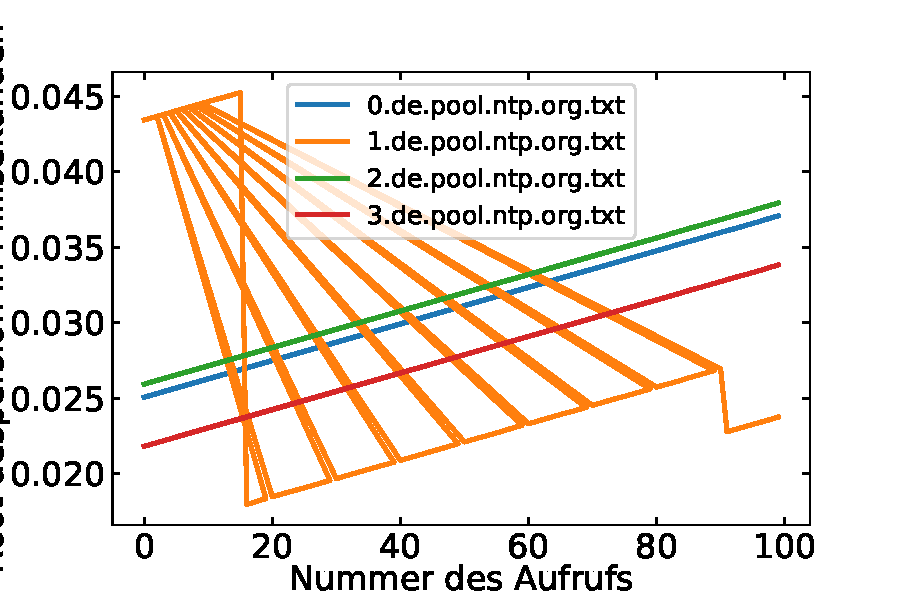
\includegraphics[width=\textwidth]{root_despersion_all.pdf}
    \captionof{figure}{Root Dispersion von zwei Zeitservern}
    \label{fig:disp}
\end{center}

Die Root Dispersion gibt die Abweichung der Uhr des Servers zu seiner Zeitquelle an.

Auffällig ist es, dass die Messwerte im Mikrosekundenbereich immer wieder stark ausschlagen, wohingegen die Messwerte von Offset und Delay sich im Millisekundenbereich befinden und eher kontinuierlich verlaufen. Das starke Ausschlagen ist damit zu begründen, dass wir alle 8 Sekunden Messungen vorgenommen haben. Dieses Interval ist offenbar so groß, dass man die Entwicklung der Root Dispersion nicht genau nachhvollziehen kann und entweder eine Verhältnismäßig kleine oder große Root Dispersion als Messergebnis bekommt.


%     - Quellenverzeichnis -    %
%\newpage
%\printbibliography

\end{document}
